% Include-ready TikZ; compile from paper/article/ (see README.md).
% Packages: tikz, amsmath, fontenc[T1], lmodern. No TikZ libraries required.
% Final width: 152.4 mm; ordinary labels >= 8.5 pt; strokes >= 0.45 pt.
% One teal accent; position, line weight and direct labels preserve greyscale meaning.
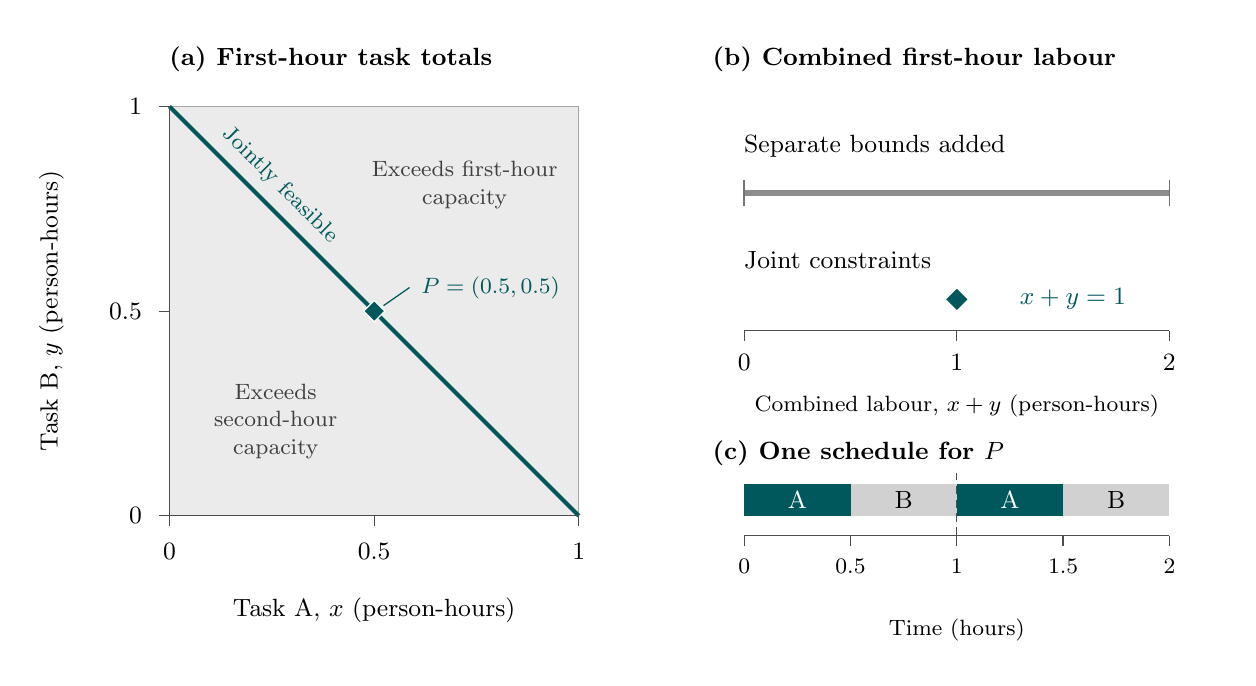
\begin{tikzpicture}[x=1mm,y=1mm,
  font=\fontsize{9}{11}\selectfont,
  every node/.style={inner sep=0pt,outer sep=0pt},
  scaxis/.style={draw=black!70,line width=0.45pt},
  scjoint/.style={draw=scaccent,line width=1.5pt},
  sctitle/.style={anchor=west,font=\fontsize{9.5}{11.5}\selectfont\bfseries},
  sccontext/.style={align=center,text=black!75,font=\fontsize{8.5}{10}\selectfont}]
  \definecolor{scaccent}{RGB}{0,88,92}
  % Generated by calculate.py; exact derived values, no graphical styling.
\def\SCMarginalMinimum{0}
\def\SCMarginalMaximum{1}
\def\SCTargetBoundary{1}
\def\SCObservationEnd{2}
\def\SCTaskTotal{1}
\def\SCSeparateTotalMinimum{0}
\def\SCSeparateTotalMaximum{2}
\def\SCJointTotal{1}
\def\SCFeasibleStart{(0,1)}
\def\SCFeasibleEnd{(1,0)}
\def\SCFeasibleMidpoint{(0.5,0.5)}
\def\SCTimelineX{0.5}
\def\SCTimelineY{0.5}
\def\SCTaskABlocks{0/0.5,1/1.5}
\def\SCTaskBBlocks{0.5/1,1.5/2}

  \path[use as bounding box] (0,0) rectangle (152.4,80);
  \node[sctitle] at (18,76) {(a) First-hour task totals};
  \node[sctitle] at (87,76) {(b) Combined first-hour labour};

  % Panel (a): the square is the Cartesian product of the separate bounds.
  \begin{scope}[shift={(18,18)},x=52mm,y=52mm]
    \fill[black!8] (\SCMarginalMinimum,\SCMarginalMinimum)
      rectangle (\SCMarginalMaximum,\SCMarginalMaximum);
    \draw[draw=black!35,line width=0.45pt]
      (\SCMarginalMinimum,\SCMarginalMinimum)
      rectangle (\SCMarginalMaximum,\SCMarginalMaximum);
    \draw[scjoint] \SCFeasibleStart -- \SCFeasibleEnd;
  \end{scope}
  \draw[scaxis] (18,70) -- (18,18) -- (70,18);
  \foreach \v in {0,0.5,1} {
    \draw[scaxis] ({18+52*\v},18) -- ({18+52*\v},16.7);
    \node[anchor=north] at ({18+52*\v},14.5) {\v};
    \draw[scaxis] (18,{18+52*\v}) -- (16.7,{18+52*\v});
    \node[anchor=east] at (14.5,{18+52*\v}) {\v};
  }
  \node at (44,6) {Task A, $x$ (person-hours)};
  \node[rotate=90] at (3,44) {Task B, $y$ (person-hours)};
  \node[sccontext,text width=27mm] at (55.5,60)
    {Exceeds first-hour\\capacity};
  \node[sccontext,text width=27mm] at (31.5,30)
    {Exceeds second-hour\\capacity};
  \node[rotate=-45,text=scaccent,font=\fontsize{8.5}{10}\selectfont]
    at (32,60) {Jointly feasible};
  \path[fill=scaccent,draw=white,line width=0.45pt]
    (44,45.35) -- (45.35,44) -- (44,42.65) -- (42.65,44) -- cycle;
  \draw[draw=scaccent,line width=0.45pt] (45.2,44.7) -- (48.5,47);
  \node[anchor=west,text=scaccent,font=\fontsize{8.5}{10}\selectfont]
    at (50,47) {$P=(\SCTimelineX,\SCTimelineY)$};

  % Panel (b): linear projection (x,y) -> x+y on a common 0--2 scale.
  \node[anchor=west] at (91,65) {Separate bounds added};
  \draw[draw=black!45,line width=2pt]
    ({91+27*\SCSeparateTotalMinimum},59)
    -- ({91+27*\SCSeparateTotalMaximum},59);
  \foreach \v in {\SCSeparateTotalMinimum,\SCSeparateTotalMaximum} {
    \draw[draw=black!55,line width=0.65pt]
      ({91+27*\v},57.4) -- ({91+27*\v},60.6);
  }
  \node[anchor=west] at (91,50.5) {Joint constraints};
  \path[fill=scaccent] ({91+27*\SCJointTotal},46.85)
    -- ++(1.35,-1.35) -- ++(-1.35,-1.35) -- ++(-1.35,1.35) -- cycle;
  \node[anchor=west,text=scaccent] at (126,45.5)
    {$x+y=\SCJointTotal$};
  \draw[scaxis] (91,41.5) -- (145,41.5);
  \foreach \v in {0,1,2} {
    \draw[scaxis] ({91+27*\v},41.5) -- ({91+27*\v},40.2);
    \node[anchor=north] at ({91+27*\v},38.5) {\v};
  }
  \node[font=\fontsize{8.5}{10}\selectfont] at (118,32)
    {Combined labour, $x+y$ (person-hours)};

  % Panel (c): each thick interval is a quantitative time mark, not a node.
  % The arbitrary within-hour switches construct one witness for the point P.
  \node[sctitle] at (87,26) {(c) One schedule for $P$};
  \foreach \start/\finish in \SCTaskABlocks {
    \draw[draw=scaccent,line width=4mm,line cap=butt]
      ({91+27*\start},20) -- ({91+27*\finish},20);
    \node[text=white] at ({91+27*(\start+\finish)/2},20) {A};
  }
  \foreach \start/\finish in \SCTaskBBlocks {
    \draw[draw=black!18,line width=4mm,line cap=butt]
      ({91+27*\start},20) -- ({91+27*\finish},20);
    \node at ({91+27*(\start+\finish)/2},20) {B};
  }
  \draw[scaxis,densely dashed] (118,15.5) -- (118,23.5);
  \draw[scaxis] (91,15.5) -- (145,15.5);
  \foreach \v in {0,0.5,1,1.5,2} {
    \draw[scaxis] ({91+27*\v},15.5) -- ({91+27*\v},14.2);
    \node[anchor=north,font=\fontsize{8.5}{10}\selectfont]
      at ({91+27*\v},12.5) {\v};
  }
  \node[font=\fontsize{8.5}{10}\selectfont] at (118,3.5) {Time (hours)};
\end{tikzpicture}%
